\documentclass[a4paper,12pt]{ctexbook}
\usepackage[margin=2cm]{geometry}
\usepackage{graphicx}
\usepackage{subfigure}
\usepackage{amsmath}
\usepackage{float}
\usepackage[colorlinks,linkcolor=black]{hyperref}%colorlinks启用链接颜色,linkcolor指定对应的颜色
\pagestyle{empty}
\begin{document}

\begin{center}
\huge \textbf{R学习}
\end{center}

\tableofcontents
\newpage
\begin{flushleft}

\chapter{准备}
\section{R语言介绍}
R语言和其他的语言之间提供了非常好的接口。
\begin{itemize}
  \item R语言对大小写敏感。
  \item 基本的命令是表达式或者赋值。
  \item 命令可以被;隔开。
  \item 注释符号用\#
\end{itemize}

%暂时没有理解这句话。
R的缺点:
\begin{itemize}
  \item 耗内存,所以要用rm命令来删除对象,以释放内存,如:\verb|rm(x,y,z)|。
  \item 精度有问题
\end{itemize}

\section{R命令介绍}
在linux下面使用R的时候,我们一般用到的命令是:
\begin{verbatim}
R --vanilla <plot.R > a.out
\end{verbatim}
这里的 --vanilla 是参数,当然还有别的很多参数,具体有兴趣可以用man命令查看。
<plot.R 的意思是将plot-R这个文件作为一个输入。既然有输入,那自然有输出,>a.out 的意思就是将显示的内容输出到a.out这个文件中。

\section{关于包的安装与使用}
\subsection{安装对应的包}
R语言中,有多种方式可以导入数据包,如下,一目了然:
\begin{verbatim}
library(Hmisc)
source("plotter.R")
\end{verbatim}
如果没有对应的包,就要安装,其中source("plotter.R"),这个plotter.R文件是在当前的目录下的。
在linux下,进入R之后,用如下命令:
\begin{verbatim}
install.packages("ggplot2")
install.packages("Hmisc")
\end{verbatim}
\subsection{包的使用}
用source命令导入包,如:\verb|>source("plot.R")|

\section{查看帮助}
如查看solve的帮助:
\begin{itemize}
  \item \verb|>help(solve)|
  \item \verb|>?solve|
\end{itemize}
对于一些特殊的字符串可以加上双引号,如: \verb|>help("[[")|

\chapter{基础语法}
mode(X)\#可以查看变量的类型


\section{算术操作和向量运算}
创建含有5个值的向量x:\\
\begin{itemize}
	\item \verb|x<-c(10,2.5,3.4,2,6,1)|
	\item \verb|x=c(10,2.5,3.4,2,6,1)|
	\item \verb|assign("x",c(10,2.5,3.4,2,6,1))|
	\item \verb|c(10,2.5,3.4,2,6,1)->x|
\end{itemize}
下面是一些简单的应用:
\begin{itemize}
	\item \verb|1\x|\#显示x的倒数。
	\item \verb|y<-c(x,0,x)|\#创建y向量。
	\item \verb|v<-2*x+y+1|\#
\end{itemize}

接下来是一些常用的数学函数:
\begin{description}
	\item[log(X)] log函数
	\item[exp(X)] 以e为底的指数函数
	\item[sin(X)] sin
	\item[cos(X)] cos
	\item[tan(X)] tan
	\item[sqrt(X)] 对里面的数开根号
	\item[max(X)]
	\item[min(X)]
	\item[length(X)]
	\item[sum(X)]
	\item[prod(X)] 得到向量中所有数的乘积
	\item[mean(X)] 得到均值
	\item[var(X)] 得到方差
	\item[sort(X)] 对X进行排序
	\item[rev(X)] 颠倒向量
	\item[sd(X)] 得到标准差
%	\item[] describe
\end{description}
\section{向量的组合}
X1=c(1,2,3,4)\\
X2=c(5,6,7,8)

rbind(X1,X2)\#得到一个排列的矩阵
$$\begin{bmatrix}
	1&2&3&4 \\
	5&6&7&8 
\end{bmatrix}$$
cbind(X1,X2)\#另一种排列方式	
$$\begin{bmatrix}
1&5\\
2&6\\
3&7\\
4&8
\end{bmatrix}$$

\section{字符和字符向量}
字符向量既可以用双引号也可以使用单引号。

\verb|\n|\#换行
\verb|\t|\#制表符
\verb|\b|\#退格

c()可以将几个字符向量链接成一个字符向量。\\
paste()可以进行任意的链接。

letters,这是一个特殊的向量,里面包含26个字母。例如letters[2]='b'

\section{关于正则序列}
1:30等价于c(1,2,...,29,30)\#请注意,冒号:的优先级别是最高的。\\
30:1也是同样的道理,可以产生逆向序列。

seq(2,100,by=2)\#指定公差,表示(2,4,...,98,100),by就公差的意思。\\
seq(5,121,length=10)\#指定长度。

a[i]表示a向量中的第i个元素。\\
a[2,3,4]无法显示,报错如下:\verb|Error in a[2, 4] : incorrect number of dimensions|\\
a[2:4]表示a向量中第二和到第四个元素,返回的是一个3个数值的向量。

a[-1]表示第一个不显示。\\
a[-(1:3)]表示第一个到第三个不显示。

\section{一些奇怪的函数}
函数is.na(X1)表示返回一个和X1长度相同的向量,里面的值为FALSE。

which.max(a)\#显示a向量中最大值的下标,不可以用对字符向量进行该操作。\\
which.min(a)

\section{矩阵的操作}
\subsection{生成矩阵}
a1=c(1:12)\\
matrix(a1,nrow=3,ncol=4),\\
matrix(a1,nrow=3,ncol=4,byrow=T)显示如下:
\begin{verbatim}
> a1<-c(1:12)
> a1
[1]  1  2  3  4  5  6  7  8  9 10 11 12
> matrix(a1,nrow=3,ncol=4)
[,1] [,2] [,3] [,4]
[1,]    1    4    7   10
[2,]    2    5    8   11
[3,]    3    6    9   12
> matrix(a1,nrow=3,ncol=4,byrow=T)
[,1] [,2] [,3] [,4]
[1,]    1    2    3    4
[2,]    5    6    7    8
[3,]    9   10   11   12
\end{verbatim}
\subsection{矩阵加减法}
\subsection{矩阵的转置}
t(a1)\#表示a1矩阵的转置矩阵,在下面的矩阵乘法中进行测试。
\subsection{矩阵乘法}
\verb|a*b|注意和下面的区别,这里的意思是矩阵每个元素的乘积,所以这里的操作只能是相同阶数的矩阵进行操作。
\verb|a%*%b|注意,中间没有空格。
\begin{verbatim}
> a1*a1
[,1] [,2] [,3] [,4]
[1,]    1   16   49  100
[2,]    4   25   64  121
[3,]    9   36   81  144
> a1%*%a1
[,1]
[1,]  650
> a1%*%t(a1)
[,1] [,2] [,3] [,4] [,5] [,6] [,7] [,8] [,9] [,10] [,11] [,12]
[1,]    1    2    3    4    5    6    7    8    9    10    11    12
[2,]    2    4    6    8   10   12   14   16   18    20    22    24
[3,]    3    6    9   12   15   18   21   24   27    30    33    36
[4,]    4    8   12   16   20   24   28   32   36    40    44    48
[5,]    5   10   15   20   25   30   35   40   45    50    55    60
[6,]    6   12   18   24   30   36   42   48   54    60    66    72
[7,]    7   14   21   28   35   42   49   56   63    70    77    84
[8,]    8   16   24   32   40   48   56   64   72    80    88    96
[9,]    9   18   27   36   45   54   63   72   81    90    99   108
[10,]   10   20   30   40   50   60   70   80   90   100   110   120
[11,]   11   22   33   44   55   66   77   88   99   110   121   132
[12,]   12   24   36   48   60   72   84   96  108   120   132   144
\end{verbatim}

\subsection{矩阵的其他操作}
diag(a1)\#这就一个关于对角操作的命令,这里返回a1矩阵的对角,返回的是一个一维向量。
diag(3)\#生成一个对角线为1的3阶矩阵。
\begin{verbatim}
> a1
[,1] [,2] [,3] [,4]
[1,]    1    4    7   10
[2,]    2    5    8   11
[3,]    3    6    9   12
> diag(a1)
[1] 1 5 9
> diag(5)
[,1] [,2] [,3] [,4] [,5]
[1,]    1    0    0    0    0
[2,]    0    1    0    0    0
[3,]    0    0    1    0    0
[4,]    0    0    0    1    0
[5,]    0    0    0    0    1
\end{verbatim}

\subsection{解矩阵方程的方法}
slove(a1)\#求矩阵的逆矩阵。但是有问题,可能是参数的错误。总之解方程就是使用这个函数。

\subsection{将向量转换成数组}
dim(X1)<-c(2,3)\#会报错,暂时不清楚原因。
\begin{verbatim}
> dim(X1)<-c(2,3)
Error in dim(X1) <- c(2, 3) : object 'X1' not found
> dim(a1)<-c(2,3)
Error in dim(a1) <- c(2, 3) : 
dims [product 6] do not match the length of object [12]
\end{verbatim}

\section{vector, array, matrix之间的联系}
vector是一维的,array是多维的,matrix是二维表单。


\section{数据的处理}
data.frame\\
构建数据框的步骤如下:\\
x1=seq(2,12,by=2)\\
x2=1:6\\
xf=data.frame(x1,x2)
\begin{verbatim}
> x1=seq(2,12,by=2)
> x2=1:6
> xf=data.frame(x1,x2)
> xf
x1 x2
1  2  1
2  4  2
3  6  3
4  8  4
5 10  5
6 12  6
> t(xf)
[,1] [,2] [,3] [,4] [,5] [,6]
x1    2    4    6    8   10   12
x2    1    2    3    4    5    6
\end{verbatim}
\subsection{从外部读入数据}
x=read.table("a.txt")\#这里的x是一个数据框(Frame),可以指定路径,也可以放在工作目录。
\subsection{从剪切板读入数据}
y=read.table("clipboard",header=F)
\subsection{从EXCEL读取文件}
将EXCEL文件另存为prn格式(以空格分割数据)。y=read.table("a.prn",header=T)\\
将EXCEL文件另存为csv格式。y=read.table("a.csv",header=T)\\

直接读取xls文件的方法:\\
安装RODBC包\\
\verb|>library(RODBC)|\\
z<-odbcConnectExcel("test.xls")\\
w<-sqlFetch(z,"Sheet1")

\section{画图}
高水平画图函数只该函数本身就能作图,低水平画图函数要借助别的命令才能画一个完成的图。

\subsection{散点图}
散点图可以用于线性回归:\\
\verb|plot(x1,x2)|\\
\verb|plot(x$x1,x$x2)|
\begin{verbatim}
plot(x$x1,x$x2)
main="this is title"
xlab="x轴title"
ylab="y轴title"
xlim=c(0,100)
ylim=c(0,100)
xaxs="i"
yaxs="i"
col="red"
pch=19 #表示点的款式
\end{verbatim}

\subsection{连线图}
\begin{verbatim}
a=2:6
b=4:8
plot(a,b,type="l")
\end{verbatim}

\subsection{直方图}
\verb|hist(x$x1)|

\subsection{柱状图}
\verb|table(x$x1)|\\
\verb|barplot(table(x$x1))|

\subsection{饼图}
\verb|table(x$x1)|

\subsection{分布函数的密度图}
plot(density(rnorm(1000)))

\subsection{地图,绘制地理数据}
map("world",fill=TRUE,col=heat.color(10))\\
map("stata",boundary=FALSE,col="red",odd=TRUE)


\section{编写R脚本语法}
\subsection{编写脚本}
编写的脚本以*.R命名,在导入的时候使用source命令导入。\\
\verb|>source("D:\\h.R")|

\subsection{产生随机数}
产生随机数要用到分布函数。\\
x1=round(runif(100,min=80,max=100))

x1=round(morm()),使用不同的分布参数,得到的结果不一样。
\begin{description}
	\item[rpois] 泊松分布
	\item[rexp] 指数分布
	\item[rgamma] Gamma分布
	\item[rbinom] 二项分布
	\item[rgeom] 几何分布
\end{description}

\subsection{循环语句}
for(i in 1:59){a[i]=i*3+3}\\

a[i]=5;\\
i=1;\\
while(a[i]<121){i=i+1;a[i-1]+2}


\chapter{NorNet画图脚本分析}
\section{基础实验脚本分析}
首先上图:
\begin{figure}[H]
	\begin{center}
	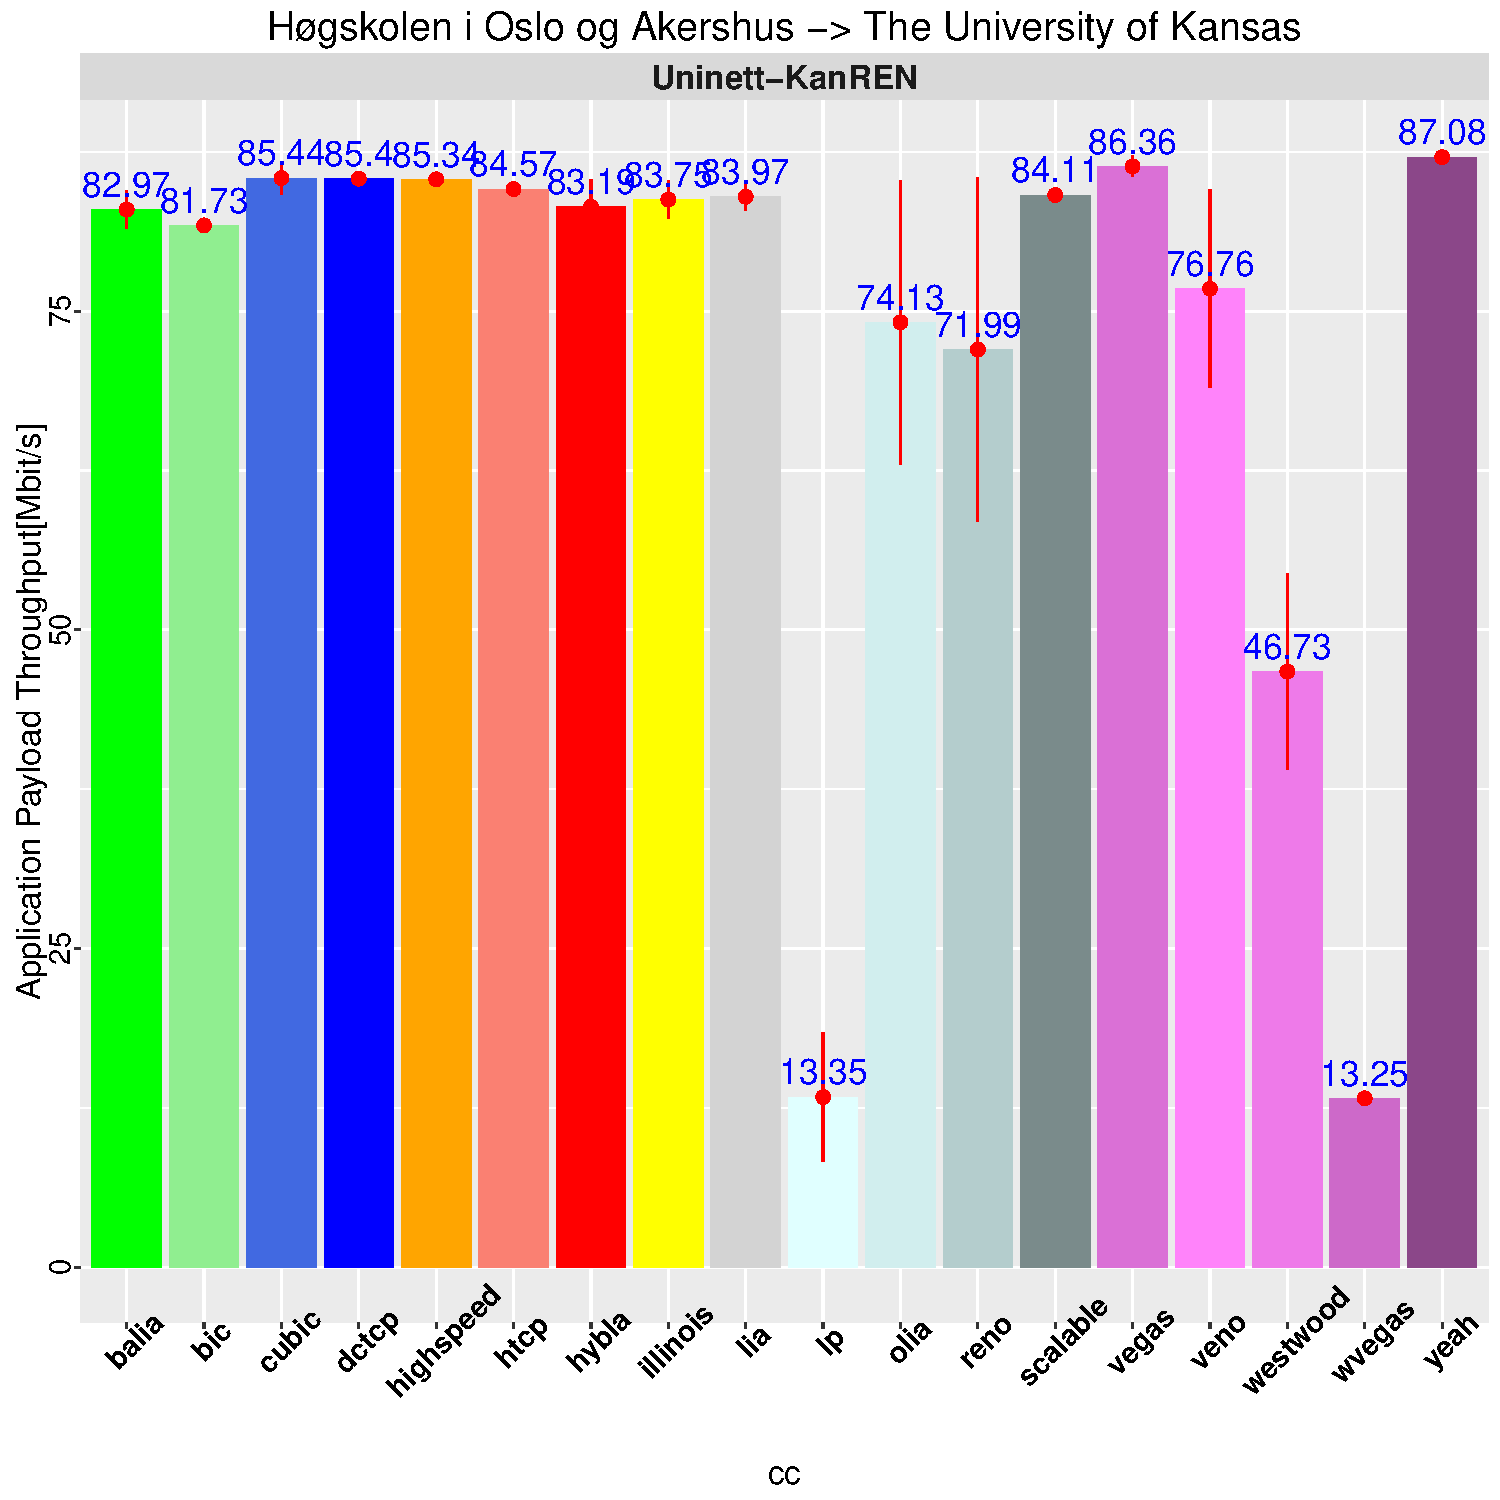
\includegraphics[width=10cm]{NorNet示例/demo-hioa-ku/hioa-ku-IPv6.pdf}
	\caption{基础实验脚本}
	\end{center}
\end{figure}
首先看一下画出这张图的源脚本:
\begin{verbatim}
library(ggplot2)
library(Hmisc)
source("plotter.R")#导入包的两种方式
name <- "hioa-ku"

# Specification of the x-axis sorting order:
allResults <- loadResults("passive.flow-ReceivedBitRate.data.bz2")
allResults <- subset(allResults,allResults$CMT == 'off')

allResults$IPVersion <- factor(allResults$IPVersion,levels=c("4","6"))

plotColours <- c("green","lightgreen","royal blue","blue", "orange","salmon","red","yellow","lightgray","lightcyan","lightcyan2","lightcyan3","lightcyan4","orchid","orchid1","orchid2","orchid3","orchid4")

for(ipversion in c(6))
{
allResultsSubset <- subset(allResults,allResults$IPVersion == ipversion)
pdf(paste(sep="", name,"-IPv",ipversion,".pdf"), width=10, height=10, family="Helvetica", pointsize=22)

numberOfRuns <- length(levels(factor(allResultsSubset$TimeStamp)))
title <- paste(sep="", levels(factor(allResults$FromSite)), " -> ", levels(factor(allResults$ToSite)))

xSet <- allResultsSubset$CC
xTitle <- "cc"
ySet <- allResultsSubset$passive.flow.ReceivedBitRate/(1024*1024)
yTitle <- "Application Payload Throughput[Mbit/s]"
zSet <- sprintf("%s-%s",allResultsSubset$FromProvider,allResultsSubset$ToProvider)
zTitle <- "From Provider{F}"
xAxisTicks <- getIntegerTicks(xSet)   # Set to c() for automatic setting
yAxisTicks <- getIntegerTicks(ySet)   # Set to c() for automatic setting
hset<-data.frame(CC=xSet,ReceivedBitRate=ySet,Path=zSet)

p <- ggplot(hset,aes(x=CC,y=ReceivedBitRate,fill=CC))+scale_fill_manual(values = plotColours)
p <- p + labs(title=title,fill=zTitle,x=xTitle,y=yTitle)

# Theme (see http://docs.ggplot2.org/0.9.2.1/theme.html for options):
p <- p + theme(title = element_text(size=16),
axis.title      = element_text(size=16),
strip.text      = element_text(size=16, face="bold"),
axis.text.x     = element_text(size=14, angle=45, face="bold", colour="black"),
axis.text.y     = element_text(size=14, angle=90, hjust=0.5, colour="black"),
legend.position = "none")
p <- p + facet_grid(~Path) + 
stat_summary(fun.y=mean, geom='bar', size=3)

# Add confidence intervals:
# NOTE: Needs at least 2 (*two*) runs to work!
if(numberOfRuns >= 2) {
p <- p + stat_summary(fun.data=mean_cl_boot, geom='pointrange', colour="red")
}

p <- p + stat_summary(aes(label=round(..y..,2)), fun.y=mean, geom="text",
colour='blue', size=6, vjust = -0.5)

print(p)
}
dev.off()
\end{verbatim}

\section{缓存分析图}
上图:
\begin{figure}[H]
	\begin{center}
		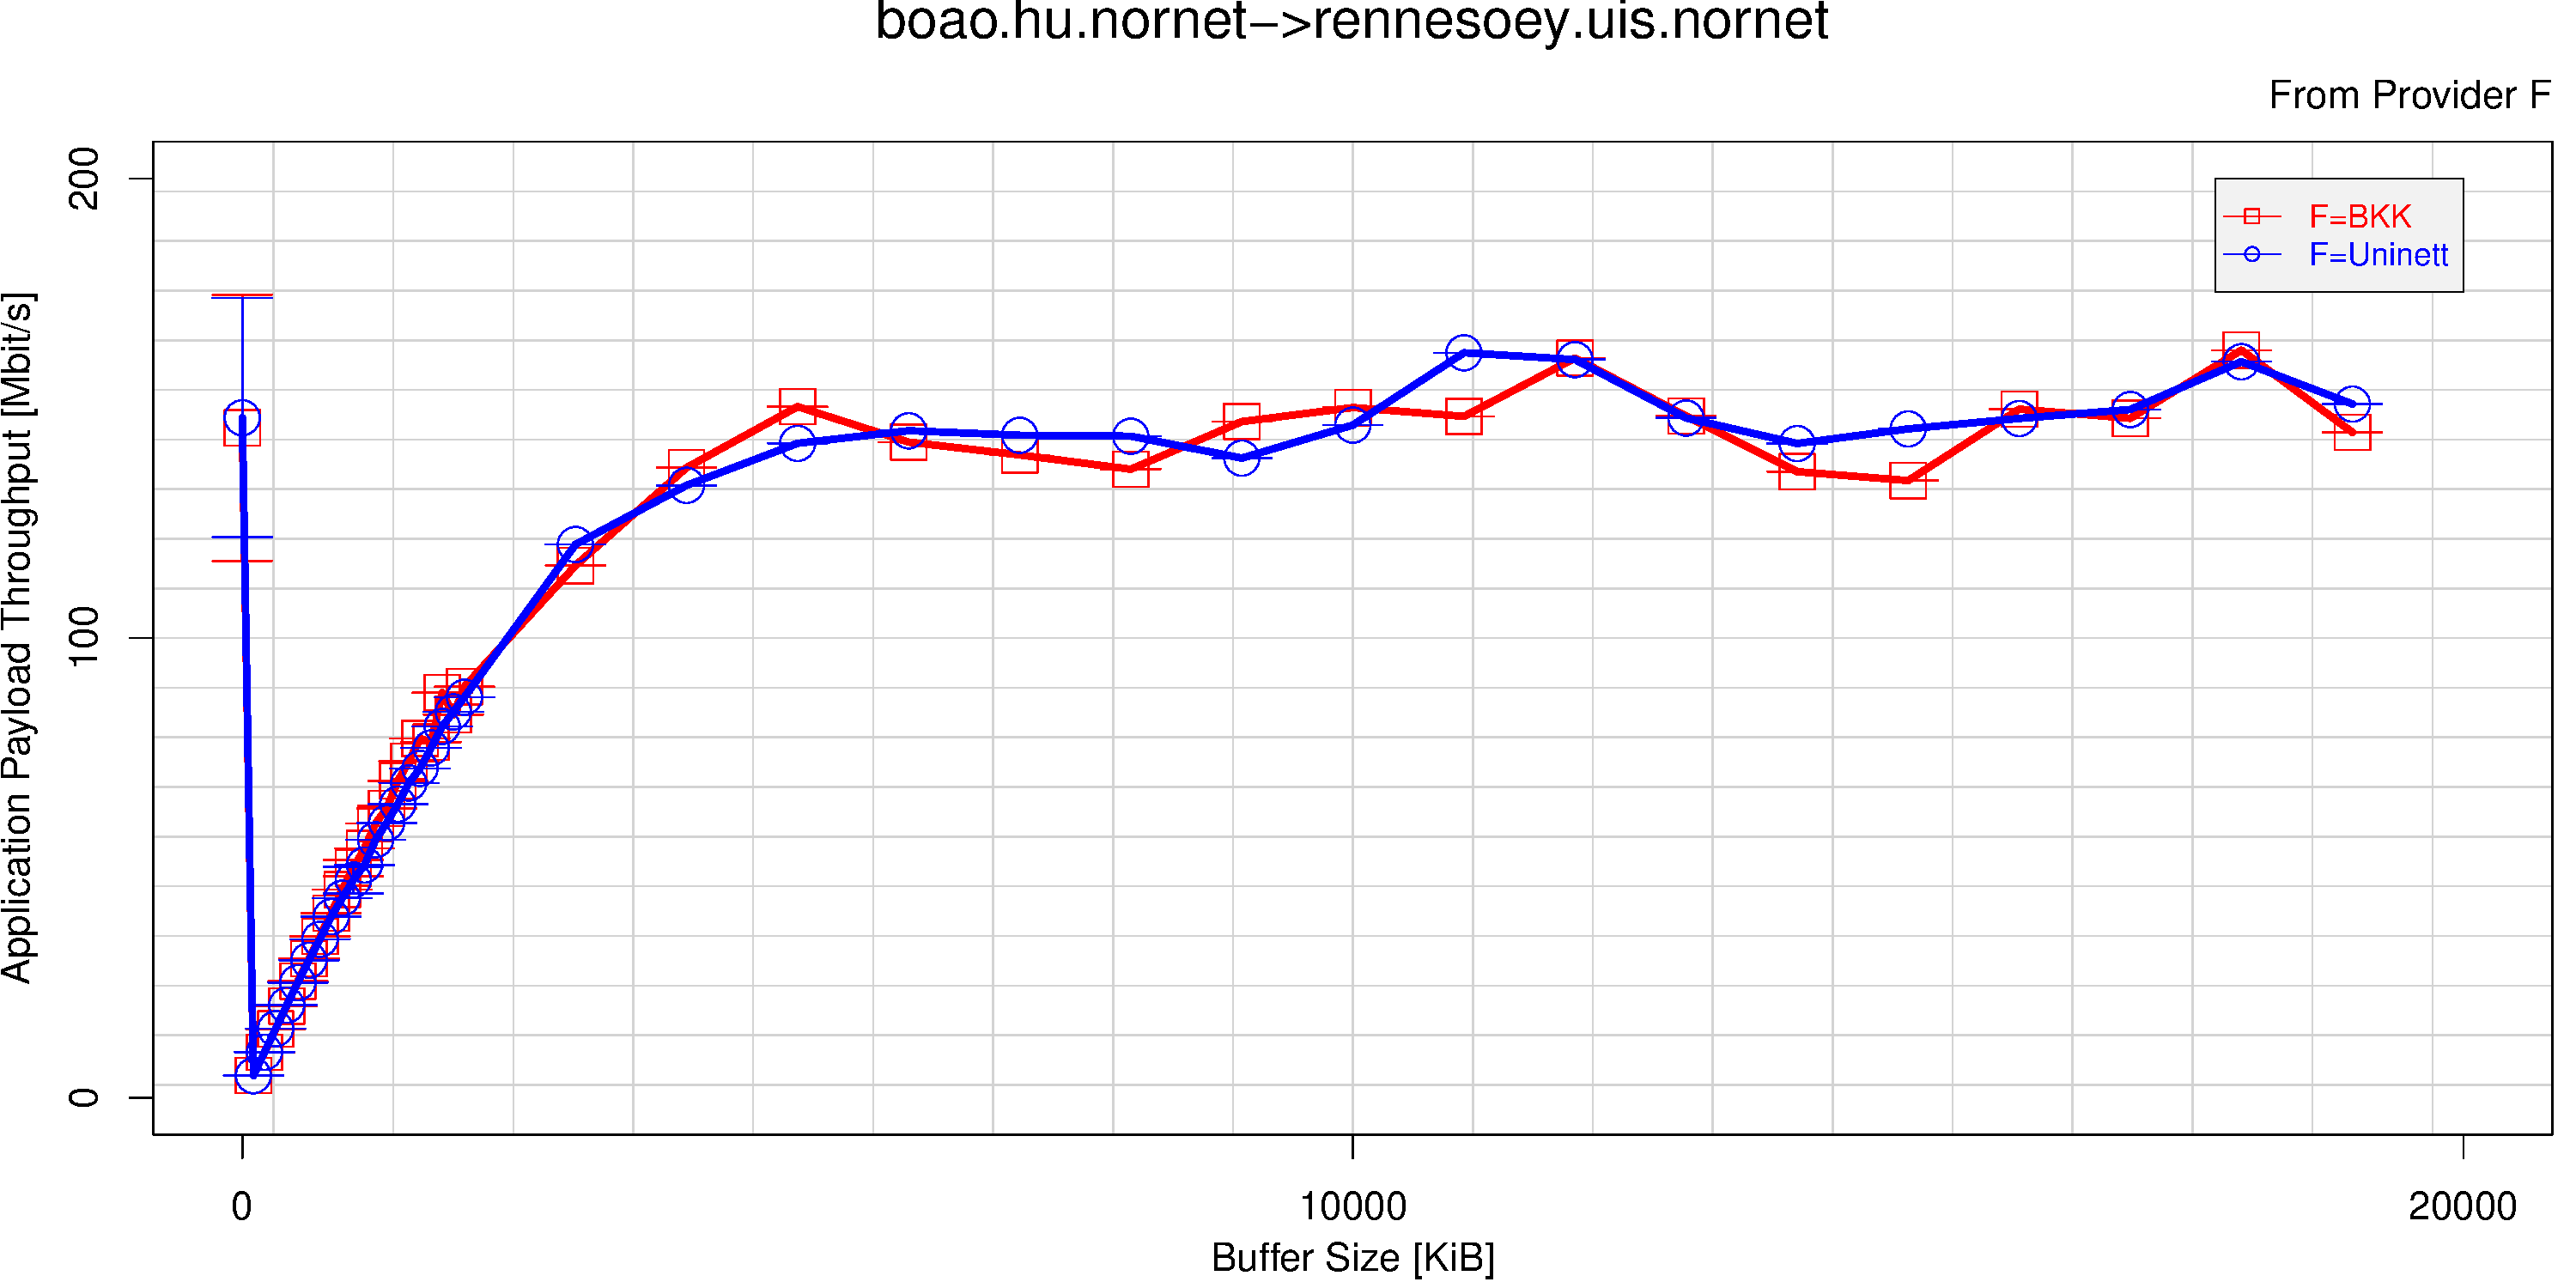
\includegraphics[width=10cm]{NorNet示例/hybla-buffer-uib-ku缓冲模型/hybla-buffer.pdf}
		\caption{缓存趋势脚本}
	\end{center}
\end{figure}
本图的源脚本如下:
\begin{verbatim}
source("plotter.R")

name <- "hybla-buffer-v6"
title <- "boao.hu.nornet->rennesoey.uis.nornet"

data <- loadResults(paste(sep="", name, "/passive.flow-ReceivedBitRate.data.bz2"))

xSet <- data$SndBufSize / 1024
xTitle <- "Buffer Size[KiB]"

ySet <- data$passive.flow.ReceivedBitRate / (1024 * 1024)
yTitle <- "Application Payload Throughput[Mbit/s]"

zSet <- data$FromProvider
zTitle <- "From Provider{F}"
vSet <- data$ToProvider
vTitle <- "To Provider{T}"
wSet <- c()
wTitle <- ""

aSet <- data$CMT
aTitle <- "CMT{:Psi:}"
bSet <- data$FromSite
bTitle <- "Source"

pSet <- data$CC
pTitle <- "Congestion Control{:varphi:}"

xAxisTicks <- getIntegerTicks(xSet)   # Set to c() for automatic setting
yAxisTicks <- getIntegerTicks(ySet)   # Set to c() for automatic setting
dotSet <- 0:18
legendPos <- c(1,1)

pdf(paste(sep="", name, ".pdf"), width=20, height=10, family="Helvetica", pointsize=22)
plotstd6(title,
pTitle, aTitle, bTitle, xTitle, yTitle, zTitle,
pSet, aSet, bSet, xSet, ySet, zSet,
vSet, wSet, vTitle, wTitle,
xAxisTicks=xAxisTicks,
yAxisTicks=yAxisTicks,
dotSet=dotSet,
type="l",
colorMode=cmColor,
hideLegend=FALSE,
legendPos=legendPos,
pStart=0)
dev.off()
\end{verbatim}

\section{IPv4和IPv6的比较图表}
\begin{figure}[H]
	\begin{center}
		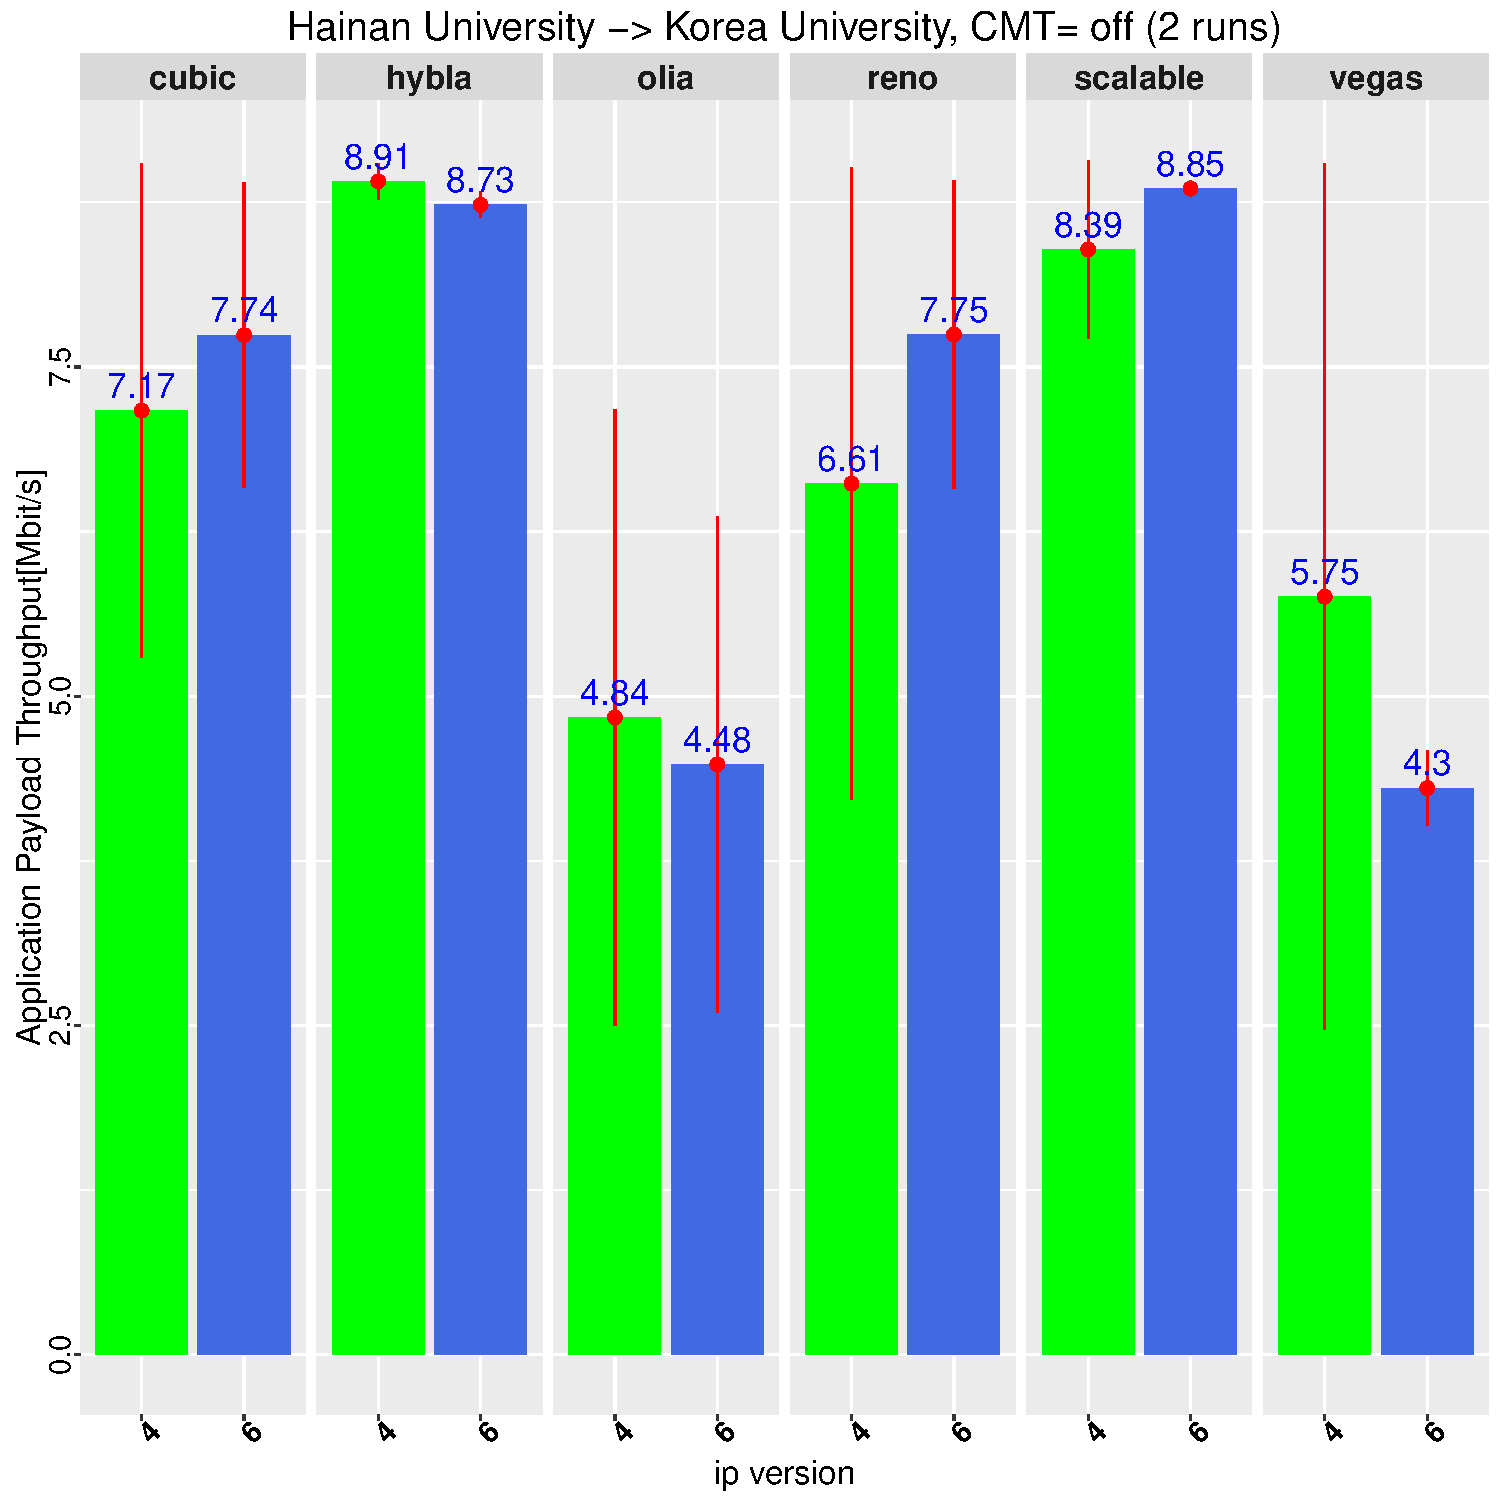
\includegraphics[width=10cm]{NorNet示例/vc-hu-korea/hu-koreavc-mptcp-CERNET.pdf}
		\caption{IPv4和IPv6的比较分析}
	\end{center}
\end{figure}
\begin{verbatim}
library(ggplot2)
library(Hmisc)
source("plotter.R")

name <- "hu-korea"
cmt <- "off"
localetho <- "CERNET"


# Specification of the x-axis sorting order:
allResults <- loadResults(paste(sep="", name, "/passive.flow-ReceivedBitRate.data.bz2"))
allResults$IPVersion <- factor(allResults$IPVersion,levels=c("4","6"))

plotColours <- c("green","royal blue", "blue", "orange","salmon","red",'yellow')

allResults$IPVersion <- factor(allResults$IPVersion,levels=c("4","6"))

numberOfRuns <- length(levels(factor(allResults$TimeStamp)))

allResults <- subset(allResults,FromProvider== localetho)

pdf(paste(sep="", name,"vc-",cmt,"-",localetho,".pdf"), width=10, height=10, family="Helvetica", pointsize=22)

#for(cmt in levels(factor(allResults$CMT))) 
#{
allResultsSubset <- subset(allResults, (allResults$CMT == cmt))

title <- paste(sep="", levels(factor(allResults$FromSite)), " -> ", levels(factor(allResults$ToSite)),
", CMT= off (", numberOfRuns , " runs)")

xSet <- allResultsSubset$IPVersion
xTitle <- "ip version"

ySet <- allResultsSubset$passive.flow.ReceivedBitRate/(1024*1024)
yTitle <- "Application Payload Throughput[Mbit/s]"

#zSet <- sprintf("%s-%s",allResultsSubset$FromProvider,allResultsSubset$ToProvider)
#zTitle <- "From Provider{F}"
zSet <- sprintf("%s",allResultsSubset$CC)
zTitle <- "From Provider{F}"



xAxisTicks <- c()
yAxisTicks <- c()
#xAxisTicks <- getIntegerTicks(xSet)   # Set to c() for automatic setting
#yAxisTicks <- getIntegerTicks(ySet)   # Set to c() for automatic setting


hset<-data.frame(CC=xSet,ReceivedBitRate=ySet,Path=zSet)

p <- ggplot(hset,
aes(x=CC,y=ReceivedBitRate,fill=CC)) +
scale_fill_manual(values = plotColours)
p <- p + labs(title=title,
fill=zTitle,
x=xTitle,
y=yTitle)
# Theme (see http://docs.ggplot2.org/0.9.2.1/theme.html for options):
p <- p + theme(title           = element_text(size=16),
axis.title      = element_text(size=16),
strip.text      = element_text(size=16, face="bold"),
axis.text.x     = element_text(size=14, angle=45, face="bold", colour="black"),
axis.text.y     = element_text(size=14, angle=90, hjust=0.5, colour="black"),
legend.position = "none")
p <- p + facet_grid(~Path) + 
stat_summary(fun.y=mean, geom='bar', size=3)

# Add confidence intervals:
# NOTE: Needs at least 2 (*two*) runs to work!
if(numberOfRuns >= 2) {
p <- p + stat_summary(fun.data=mean_cl_boot, geom='pointrange', colour="red")
}

# All values as text:
# p <- p + geom_text(aes(label=sprintf("%1.1f", ReceivedBitRate)),
#                    vjust=1.5,colour='blue',position=position_dodge(.9),size=6)
# Only mean value as text:
p <- p + stat_summary(aes(label=round(..y..,2)), fun.y=mean, geom="text",
colour='blue', size=6, vjust = -0.5)

print(p)
#}
dev.off()	
\end{verbatim}



\end{flushleft}
\end{document}
